\documentclass[t, aspectratio=169]{beamer}
\usepackage{amsmath,amsfonts,amsthm,amstext,amssymb, xcolor, tikz, pgf, mathrsfs, polynom, pifont, tabto}

% ----------------------------------------------------------
% Theme Setup

% Use Metropolis Theme
\usetheme[numbering=fraction]{metropolis}
\setbeamertemplate{blocks}[rounded][shadow=false]
\makeatletter
\setlength{\metropolis@titleseparator@linewidth}{1pt}
\makeatother

% Define Colors
\definecolor{chargerblue}{HTML}{002764}
\definecolor{chargerred}{HTML}{e02034}
\definecolor{bggray}{HTML}{d0d3d4}

% Set Colors
\setbeamercolor{title}{fg=chargerblue}
\setbeamercolor{background canvas}{bg=white}
\setbeamercolor{title separator}{fg=chargerred}
\setbeamercolor{structure}{fg=chargerblue}
\setbeamercolor{frametitle}{fg=white, bg=chargerblue}
\setbeamercolor*{normal text}{fg=chargerblue}
\setbeamercolor*{block body}{bg=bggray}
\setbeamercolor*{block title}{bg=chargerblue, fg=white}
% ----------------------------------------------------------

% ----------------------------------------------------------
% Custom Definitions, Commands, Environments, etc.

% Sets of numbers
\def\R{\mathbb{R}} % The reals
\def\N{\mathbb{N}} % The naturals
\def\Z{\mathbb{Z}} % The integers
\def\Q{\mathbb{Q}} % The rationals

% Blank space
\newcommand{\blank}[1]{\underline{\hspace{#1}}} % Blank space

% Change font colors
\newcommand{\cyan}[1]{{\color{cyan}{#1}}} % Changes font to cyan
\newcommand{\red}[1]{{\color{red}{#1}}} % Changes font to red
\newcommand{\magenta}[1]{{\color{magenta}{#1}}} % Changes font to magenta
\newcommand{\orange}[1]{{\color{orange}{#1}}} % Changes font to orange
\newcommand{\yellow}[1]{{\color{yellow}{#1}}} % Changes font to yellow
\newcommand{\violet}[1]{{\color{violet}{#1}}} % Changes font to violet
\newcommand{\green}[1]{{\color{green}{#1}}} % Changes font to green
\newcommand{\blue}[1]{{\color{blue}{#1}}} % Changes font to blue
\newcommand{\white}[1]{{\color{white}{#1}}} % Changes font to white

% Fitted inclusion symbols
\newcommand{\fp}[1]{\left({#1}\right)} % Fitted parentheses around content
\newcommand{\fb}[1]{\left[{#1}\right]} % Fitted brackets
\newcommand{\lhoi}[1]{\left({#1}\right]} % Left half-open interval
\newcommand{\rhoi}[1]{\left[{#1}\right)} % Right half-open interval
\newcommand{\set}[1]{\left\{{#1}\right\}} % Fitted braces (useful for sets)
\newcommand{\av}[1]{\left|{#1}\right|} % Fitted absolute value bars

% Augmented Matrix Environment
\newenvironment{amatrix}[1]{%
	\left[\begin{array}{@{}*{#1}{c}|c@{}}
	}{%
	\end{array}\right]
}

% Miscellaneous
\def\then{\Rightarrow}
\def\to{\rightarrow}
\def\d{^{\circ}}
\newcommand{\?}{\stackrel{?}{=}}
\newcommand{\cmark}{\text{ \ding{51}}}
\newcommand{\xmark}{\text{ \ding{55}}}

% Coordinate Plane (Four-Quadrant)
\def\coordplane {
	\begin{tikzpicture}        \draw[step=0.25cm,black,very thin,opacity=0.25] (-2.5cm, -2.5cm) grid (2.5cm, 2.5cm);
		\draw[<->,thick,black] (-2.5cm, 0) -- (2.5cm, 0) node[anchor=north west,pos=0.94,font=\scriptsize]{$x$};
		\draw[<->,thick,black] (0,-2.5cm) -- (0, 2.5cm) node[anchor=south east,font=\scriptsize,pos=0.94]{$y$};
	\end{tikzpicture}
}

% Coordinate Plane (One-Quadrant)
\def\onequad {
	\begin{tikzpicture}
		\draw[step=0.25cm, black, very thin, opacity=0.25] (0,0) grid (7.5cm,5cm);
		\draw[->, thick, black] (0,0) -- (7.5cm, 0) node[anchor=north west,font=\scriptsize,pos=0.94]{$x$};
		\draw[->, black, thick] (0,0) -- (0,5cm) node[anchor=south east,font=\scriptsize,pos=0.94]{$y$};
	\end{tikzpicture}
}
% ----------------------------------------------------------

% ----------------------------------------------------------
% Presentation Information
\title[4-3]{Multiplication Rules and Conditional Probability}
\subtitle{Section 4-3}
\author{Jacob Ayers}
\institute{Lesson \#11}
\date{MAT 110}
% ----------------------------------------------------------

\begin{document}
	
	% Slide 1 (Title Slide)
	\begin{frame}
		\titlepage
	\end{frame}
	
	% Slide 2 (Objectives)
	\begin{frame}{Objectives}
		\begin{itemize}
			\item Use the multiplication rules of probability to find the probabilities of ``and" statements
			\item Find conditional probabilities
			\item Find probabilities of ``at least" statements
		\end{itemize}
	\end{frame}

	\begin{frame}{Independent Events}
		Two events $A$ and $B$ are \textit{independent events} if the fact that $A$ has occurred does not affect the probability of $B$ occurring. \pause
		
		Examples of independent events: \begin{itemize}
			\item Rolling a die and getting a 5, then flipping a coin and getting tails
			\item Drawing a queen from a deck of cards, putting it back, and drawing a second card and getting a queen
			\item Getting a hit in one at-bat, then getting a hit in your next at-bat
		\end{itemize}
	\end{frame}

	\begin{frame}{Independent Events}
		Determine whether each pair of events is independent. \begin{enumerate}[a)]
			\item Rolling a die and getting an even number; rolling a die and getting a 4. \pause NO \pause
			\item Drawing a red ball out of an urn, putting it back, then drawing again and getting another red ball. \pause YES \pause
			\item Drawing a red ball out of an urn, keeping it, then drawing again and getting another red ball. \pause NO
		\end{enumerate} \pause
	
		b) and c) show the difference between sampling ``with replacement" and sampling ``without replacement."
	\end{frame}

	\begin{frame}{Multiplication Rules of Probability}
		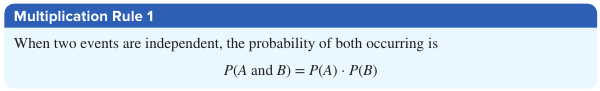
\includegraphics[width=\textwidth]{mult-1.png}
		
		\onslide<2->{Example: A coin is flipped and a die is rolled. Find the probability of getting a tail on the coin, and an even number on the die.}
		\begin{flalign*}
			\onslide<3->{P(T \text{ and even}) &= P(T) \cdot P(\text{even}) & \\}
			\onslide<4->{&= \dfrac{1}{2} \cdot \dfrac12} & \\
			\onslide<5->{&= \dfrac14 = 0.25 = 25\%}
		\end{flalign*}
	\end{frame}

	\begin{frame}{Multiplication Rules of Probability}
		Approximately 9\% of men have a type of color blindness that prevents them from distinguishing between red and green. If 3 men are selected at random, find the probability that none of them will have this type of red-green color blindness.
		
		\onslide<2->{If 9\% of men have this color blindness, then 91\% don't. So $P(\text{not colorblind}) = 0.91$.}
		\begin{flalign*}
			\onslide<3->{P(\text{none colorblind}) &= P(\text{first not and second not and third not}) & \\}
			\onslide<4->{&= P(\text{first not}) \cdot P(\text{second not}) \cdot P(\text{third not}) & \\}
			\onslide<5->{&= 0.91 \cdot 0.91 \cdot 0.91 & \\}
			\onslide<6->{&\approx 0.754}
		\end{flalign*}
	\end{frame}

	\begin{frame}{Multiplication Rules of Probability}
		An automobile salesperson finds the probability of making a sale is $0.21$. If she talks to 4 customers, find the probability that she will make 4 sales. Is this event likely or unlikely to occur?
		\begin{flalign*}
			\onslide<2->{P(\text{4 sales}) &= P(\text{sale and sale and sale and sale}) & \\}
			\onslide<3->{&= P(\text{sale}) \cdot P(\text{sale}) \cdot P(\text{sale}) \cdot P(\text{sale})} & \\
			\onslide<4->{&= (0.21)^4} & \\
			\onslide<5->{&\approx 0.002}
		\end{flalign*}
		\onslide<6->{This is a highly unlikely event; the probability is less than 0.2\%}
	\end{frame}

	\begin{frame}{Dependent Events}
		Two events $A$ and $B$ are \textit{dependent events} if the fact that $A$ has occurred affects the probability of $B$ occurring. \pause
		
		Examples of dependent events: \begin{itemize}
			\item Smoking and dying from lung cancer
			\item Having a GPA of less than 2.0 and getting a college scholarship
			\item Drawing a card from a deck, not replacing it, then drawing another card
		\end{itemize}
	\end{frame}

	\begin{frame}{Multiplication Rules of Probability}
		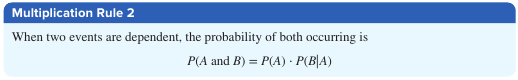
\includegraphics[width=\textwidth]{mult-2.png} \pause
		
		Note: $P(B|A)$ is the \textit{conditional probability} that $B$ will occur, given that $A$ has already occurred.
	\end{frame}

	\begin{frame}{Multiplication Rules of Probability}
		Three cards are drawn from an ordinary deck and not replaced. Find the probability that all three are jacks.
		
		\onslide<2->{Since we're not replacing the cards, the first card being a jack affects the probability that the second will be a jack. Likewise, the fact that the first two cards were jacks affects the probability that the third will be a jack.}
		\begin{flalign*}
			\onslide<3->{P(\text{3 jacks}) &= P(\text{jack and jack and jack}) & \\}
			\onslide<4->{&= P(\text{first jack}) \cdot P(\text{second jack} | \text{first jack}) \cdot P(\text{third jack} | \text{first two jacks}) & \\}
			\onslide<5->{&= \dfrac{4}{52} \cdot \dfrac{3}{51} \cdot \dfrac{2}{50} & \\}
			\onslide<6->{&\approx 0.000181}
		\end{flalign*}
	\end{frame}

	\begin{frame}{Multiplication Rules of Probability}
		Box 1 contains 2 red balls and 1 blue ball. Box 2 contains 3 blue balls and 1 red ball. A coin is tossed. If it falls heads up, a ball is drawn from Box 1. If it falls tails up, a ball is drawn from Box 2. Find the probability of a blue ball being drawn.
	\end{frame}

	\begin{frame}{Multiplication Rules of Probability}
		In a box of 12 batteries, 3 are dead. If 2 batteries are selected (without replacement) for a flashlight, find the probability that neither of them is dead. Would you say this event is likely or unlikely?
		\begin{flalign*}
			\onslide<2->{P(\text{neither dead}) &= P(\text{first not dead and second not dead}) & \\}
			\onslide<3->{&= P(\text{first not dead}) \cdot P(\text{second not dead} | \text{first not dead}) & \\}
			\onslide<4->{&= \dfrac{9}{12} \cdot \dfrac{8}{11} & \\}
			\onslide<5->{&= \dfrac{72}{132} \approx 0.545}
		\end{flalign*}
		\onslide<6->{The probability is a little above 50\%, so the event is more likely to occur than not.}
	\end{frame}

	\begin{frame}{Conditional Probability}
		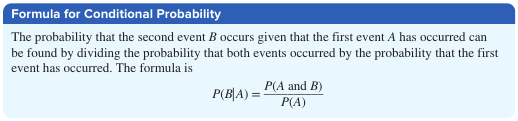
\includegraphics[width=5in]{cond-prob.png}
	\end{frame}

	\begin{frame}{Conditional Probability}
		Example: A recent survey asked 100 people if they thought women in the armed forces should be permitted to participate in combat. The results of the survey are shown.
		
		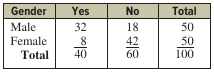
\includegraphics[width=2in]{female-mil.png}
		
		Find the probability that the respondent was male, given that the respondent answered no. \pause
		
		Let $M$ represent being a male, and $N$ represent a response of no. We need to find $P(M|N)$. \pause
		
		$P(M|N) = \dfrac{P(M \text{ and } N)}{P(N)} = \dfrac{18/100}{60/100} = \dfrac{0.18}{0.60} = 0.3$
	\end{frame}

	\begin{frame}{Conditional Probability}
		For a recent year, 0.99 of the incarcerated population is adults and 0.07 of the incarcerated are female. If an incarcerated person is selected, at random, find the probability that the person is a female given that the person is an adult.
		\begin{flalign*}
			\onslide<2->{P(F|A) &= \dfrac{P(F \text{ and } A)}{P(A)} & \\}
			\onslide<3->{&= \dfrac{0.07}{0.99} & \\}
			\onslide<4->{&\approx 0.071}
		\end{flalign*}
	\end{frame}

	\begin{frame}{Probability of ``At Least" Statements}
		When dealing with an ``at least" statement, it's often easier to find the probably of the complement and then subtract from 1.
		
		Example: The Neckware Association of America reported that 4\% of ties sold in the United States are bow ties. If 5 customers who purchased a tie are randomly selected, find the probability that at least 1 purchased a bow tie. \pause
		
		$P(\text{none}) = (0.96)^4 \approx 0.849$. \pause
		
		So $P(\text{at least one}) = 1 - P(\text{none}) = 1 - 0.849 \approx 0.151$
	\end{frame}
	
	\begin{frame}{Probability of ``At Least" Statements}
		A single die is rolled 4 times. Find the probability of getting at least one odd number. \pause
		
		$P(\text{none}) = (0.5)^4 = 0.0625$ \pause
		
		So $P(\text{at least one}) = 1 - P(\text{none}) = 1 - 0.0625 \approx 0.938$
	\end{frame}

	\begin{frame}{Next Steps}
		\begin{itemize}
			\item Complete Assignment 5
			\item Begin Module \#7 \begin{itemize}
				\item Read 4-4
				\item Watch Video Lesson \#12
			\end{itemize}
		\end{itemize}
	
		\vfill
		
		Thanks for watching!
	\end{frame}
\end{document}